\documentclass[runningheads]{llncs}

\usepackage[T1]{fontenc}
\usepackage{graphicx}
\usepackage{amsmath}
\usepackage{amssymb}
\usepackage{amsfonts}
\usepackage{quantikz}

\usepackage{float}
\begin{document}

\title{Qubit Initialization in Variational Quantum Portfolio Optimization: Effects of Circuit Depth and Objective Functions}

\titlerunning{Qubit Initialization in Variational Quantum Portfolio Optimization}
\author{Sumukh J\inst{1} \and
Tulika Dutta\inst{1}\thanks{Corresponding author}\orcidID{0000-0003-2672-5360} \and
Sapna R\inst{1}\orcidID{0000-0003-0041-9269}}

\authorrunning{S. J et al.}

\institute{Manipal Institute of Technology Bengaluru, Manipal Academy of Higher Education,
Manipal, India\\
\email{sumukh.mitblr2024@learner.manipal.edu, munai.tulika@gmail.com,sapna.r@manipal.edu}}

\maketitle

\begin{abstract}
Selecting asset allocations that jointly optimize return and downside risk remains a central challenge in computational finance. Classical exhaustive search methods become increasingly expensive as the number of binary asset-selection variables grow. This paper presents a hybrid quantum-classical variational circuit for portfolio optimization, evaluated on two problem scales viz., a seven-asset and a twelve-asset universe of U.S. equities. Hadamard and computational zero-state \emph{qubit} initialization are compared under two objective functions Expectation value and Conditional Value-at-Risk at circuit depths $d \in \{1,3\}$ for the seven-asset experiment and $d \in \{1,2,3,4\}$ for the twelve-asset experiment, across 20 independent random seeds using the Qiskit Aer simulator. Hadamard initialization achieves lower mean portfolio costs at shallow depth, though the effect diminishes as depth increases. Circuit depth has a strong effect on solution quality, while initialization does not reach statistical significance at either problem scale. The extended twelve-asset experiments ($n = 12$, 320 runs) confirm these results at scale and introduce two convergence metrics iterations-to-95\%-optimality ($T_{95}$) and 95\%-success rate ($S_{95}$) showing that deeper circuits reach near-optimal solutions in fewer iterations. Statistical significance is assessed using the Wilcoxon signed-rank test.

\keywords{variational quantum algorithms \and portfolio optimization \and qubit initialization \and CVaR \and convergence analysis}
\end{abstract}

\section{Introduction}
Selecting a portfolio that achieves an appropriate balance between expected return and financial risk remains one of the central problems in quantitative finance. Modern Portfolio Theory provides the classical mean--variance framework underlying this formulation \cite{markowitz1952}. The objective cost function $C(\mathbf{w})$ is defined as
\begin{equation}
    \mathcal{C}(\mathbf{w}) = q\mathbf{w}^\top \Sigma \mathbf{w} 
    - (1 - q)\boldsymbol{\mu}^\top \mathbf{w}
\end{equation}
where $\mathbf{w}$ is the portfolio weight vector and $q\in [0,1]$ is the risk parameter. For binary asset selection over $n$ assets, the solution space contains $2^n$ possible portfolios, rendering classical approaches computationally expensive as $n$ grows.

Quantum computing represents the $2^n$ binary asset combinations as computational basis states. A variational circuit assigns amplitudes to these states and a classical optimizer updates the circuit parameters according to the measured objective. Variational quantum algorithms therefore combine parameterized quantum circuits with classical optimization and can be evaluated using noisy hardware \cite{cerezo2021variational,preskill2018nisq}.

Choosing the initial quantum state is another design choice in a variational circuit. Two states are considered viz., the computational zero state $|0\rangle^{\otimes n}$ and the Hadamard-initialized state $|+\rangle^{\otimes n}$. The former initializes every \emph{qubit} in $|0\rangle$, whereas the latter assigns equal probability to the computational basis states before the variational layers are applied \cite{nielsen2010}. This work examines whether this difference in the starting state changes optimization performance.

\section{Motivation and Contributions}

The initial quantum state is another design choice in a variational circuit. This work examines whether starting from the computational zero state $|0\rangle^{\otimes n}$ or the Hadamard-initialized state $|+\rangle^{\otimes n}$ affects optimization performance. The comparison is made across two circuit depths in the seven-asset experiment and four depths in the twelve-asset experiment, using both Expectation and Conditional Value-at-Risk (CVaR) objectives.

The main contributions are as follows.
\begin{itemize}
    \item The effects of Hadamard and $\lvert 0\rangle$ initialization are studied under Expectation and CVaR across 20 independent random seeds.

    \item The seven-asset experiment considers circuit depths $d \in \{1,3\}$ and comprises 160 runs. The experiments are then extended to twelve assets at depths $d \in \{1,2,3,4\}$, adding 320 runs.

    \item Convergence is evaluated using two metrics: $T_{95}$, which records the first iteration at which the running-best solution reaches 95\% of the classical optimum, and $S_{95}$, which records the fraction of seeds that reach this threshold by the end of the optimization.
\end{itemize}

The remainder of this paper is organized as follows. Section~\ref{rel} reviews related work. Background concepts are introduced in Section~\ref{background}. Section~\ref{methodology} describes the methodology and experimental setup. Results and analysis are presented in Section~\ref{analysis}. Section~\ref{conclusion} concludes the paper.
\section{Related Work}\label{rel}

Portfolio optimization is studied extensively since Markowitz introduced the mean--variance framework \cite{markowitz1952}, which underlies the cost function used in the present work. Variance penalizes upward and downward deviations equally, which motivated the development of downside risk measures such as Value-at-Risk (VaR) and Conditional Value-at-Risk (CVaR) \cite{rockafellar2000}. CVaR captures the expected cost within a specified tail of the outcome distribution and is used in the present work as an alternative variational objective, with the upper-cost tail selected for minimization. The Markowitz quadratic formulation is retained for tractability, with CVaR incorporated at the objective-function level of the variational loop.

Quantum computing has also been investigated for financial optimization, including portfolio selection and broader financial applications \cite{orus2019finance,egger2020finance,kerenidis2019portfolio}. Quantum and quantum-inspired approaches have also been evaluated for dynamic portfolio optimization using real financial datasets \cite{mugel2022dynamic}. These studies establish a broader context for applying quantum optimization methods to portfolio construction, while the present work focuses specifically on initialization, circuit depth, and objective-function choice within a variational framework.

Two common approaches are used for variational optimization of combinatorial problems. QAOA uses alternating cost and mixer Hamiltonians to incorporate the structure of the optimization problem into the circuit \cite{zhou2020qaoa}. In contrast, hardware-efficient ans\"atze use parameterized rotation and entanglement layers without directly encoding the problem Hamiltonian \cite{kandala2017hardware}. The ansatz used in this work follows the hardware-efficient variational circuit approach, in which parameterized single-qubit rotations are combined with entangling gates \cite{kandala2017hardware}. This makes the choice of the initial quantum state particularly relevant, since the circuit itself does not contain problem-specific structure.

Barkoutsos et al. \cite{barkoutsos2020} show that replacing the standard expectation value with a tail-focused CVaR objective improves solution quality in variational quantum optimization. Their analysis shows that CVaR can focus the optimization on a selected tail of the sampled outcome distribution rather than averaging all outcomes into the objective. Scursulim et al. \cite{scursulim2026} show that variational quantum algorithm (VQA) performance is sensitive to circuit architecture, using a Dicke state ansatz.

A related line of work concerns parameter and state initialization in variational circuits. McClean et al.~\cite{mcclean2018barren} show that randomly initialized parameterized circuits of sufficient depth run into barren plateaus regions where the cost gradient vanishes exponentially with system size, making optimization impractical. In~\cite{Wurtz_2021_fixed_angle}, structured parameter initialization is explored, including fixed-angle heuristics for QAOA. Warm-starting provides a related approach in which information from a classical solution is incorporated into the initial quantum state \cite{egger2021warmstart}. These studies primarily address initial parameter values $\boldsymbol{\theta}_0$ rather than the initial quantum state $|\psi_0\rangle$ preceding the parameterized layers. These two forms of initialization play different roles. Parameter initialization sets the starting point in the optimization landscape, while state initialization fixes the baseline distribution on which the parameterized layers act. No prior work has compared $|0\rangle$ and Hadamard state initialization in variational quantum portfolio optimization across varying circuit depths and objective functions.
\section{Background Concepts}\label{background}
The following subsections introduce the quantum gates and circuit elements underlying the variational ansatz.
\subsection{Quantum state representation}

A \emph{qubit} is the basic unit of quantum information and can be represented as a superposition of the computational basis states ($|0\rangle$ and $|1\rangle$). Quantum gates act on these states through reversible transformations.

A general \emph{qubit} state is represented as
\begin{equation}\label{eq1}
    |\psi\rangle = \alpha|0\rangle + \beta|1\rangle,
\end{equation}
where $\alpha,\beta \in \mathbb{C}$ are probability amplitudes. The condition
\begin{equation}
    |\alpha|^2 + |\beta|^2 = 1
\end{equation}
is called the normalization equation and ensures that the total probability of measuring the \emph{qubit} is one. Equation~\ref{eq1} represents a quantum superposition state in which the \emph{qubit} simultaneously exists in both computational basis states with amplitudes $\alpha$ and $\beta$.
 
 For an $n$-\emph{qubit} system, each computational basis state $|z\rangle$ corresponds to a binary asset allocation vector,
\begin{equation}
    z_i \in \{0,1\}, \quad z_i = 1 \Rightarrow
    \text{asset } i \text{ is selected}.
\end{equation}
Thus, the $2^n$ computational basis states represent the possible binary portfolio configurations, allowing the quantum state to span the complete portfolio configuration space.

\subsection{Hadamard initialization}

The Hadamard gate is a single-\emph{qubit} quantum gate that transforms a computational basis state into a superposition of $|0\rangle$ and $|1\rangle$. Its matrix representation is
\begin{equation}
    H = \frac{1}{\sqrt{2}}
    \begin{pmatrix}
        1 & 1 \\
        1 & -1
    \end{pmatrix}.
\end{equation}
The matrix representation explicitly defines the quantum operation used to prepare the initial state in the Hadamard initialization strategy, as follows.
\begin{equation}
    H|0\rangle =
    \frac{|0\rangle + |1\rangle}{\sqrt{2}}.
\end{equation}

Applying the Hadamard gate to all $n$ \emph{qubits} initially prepared in the state $|0\rangle^{\otimes n}$ produces a uniform superposition over the $2^n$ computational basis states.
\begin{equation}
    |\psi_0\rangle =
    H^{\otimes n}|0\rangle^{\otimes n}
    =
    \frac{1}{\sqrt{2^n}}
    \sum_{z \in \{0,1\}^n}|z\rangle.
\end{equation}
Therefore, every portfolio configuration has the same measurement probability, equal to $1/2^n$.
\subsection{Parameterized $R_Y(\theta)$ Rotations}
The single-\emph{qubit} $Y$-rotation is
\begin{equation}
    R_Y(\theta) = \begin{pmatrix} 
        \cos(\theta/2) & -\sin(\theta/2) \\ 
        \sin(\theta/2) &  \cos(\theta/2) 
    \end{pmatrix},
\end{equation}
giving, for $|0\rangle$ input,
\begin{equation}
    R_Y(\theta)|0\rangle = \cos(\theta/2)|0\rangle 
    + \sin(\theta/2)|1\rangle,
\end{equation}
with measurement probability
\begin{equation}
    P(1) = \sin^2(\theta/2).
\end{equation}
Each \emph{qubit} has a trainable parameter $\theta\in[0,2\pi]$, and the full parameter vector is optimized using COBYLA.

The circuit uses $R_Y$ rotations rather than $R_X$ or general $U_3$ gates, keeping the circuit within the real-amplitude subspace. Both initialization strategies and CNOT entanglement preserve real amplitudes, so the quantum state remains within $\mathbb{R}^{2^n}$ throughout optimization.

\subsection{Entanglement via CNOT gate}
The CNOT gate is represented as follows.
\begin{equation}
    \text{CNOT} = \begin{pmatrix} 
        1 & 0 & 0 & 0 \\ 
        0 & 1 & 0 & 0 \\ 
        0 & 0 & 0 & 1 \\ 
        0 & 0 & 1 & 0 
    \end{pmatrix},
\end{equation}
The CNOT gate is applied sequentially between adjacent \emph{qubit} pairs to capture pairwise correlations.

Linear nearest-neighbor connectivity is used for hardware compatibility and lower gate overhead. The topology requires only $n-1$ CNOT gates per layer, producing shallower circuits less susceptible to noise accumulation.
\section{Methodology} \label{methodology}
This section outlines the methodology, covering problem formulation, circuit construction, objective functions, and experimental design.
\subsection{Problem Formulation}

Portfolio optimization is formulated as the problem of selecting a subset of assets that balances expected return and risk subject to the specified portfolio constraints. In this study, the problem is instantiated as a combinatorial asset selection task over $n = 7$ NASDAQ-listed equities viz., AAPL, MSFT, GOOG, AMZN, META, NVDA, and TSLA. Two years of trailing adjusted daily closing prices are retrieved using the Yahoo Finance API~\cite{yfinance}, with a rolling two-year window ending at the date of data collection in July 2026. The annualized mean return vector $\boldsymbol{\mu} \in \mathbb{R}^n$ and covariance matrix $\Sigma \in \mathbb{R}^{n \times n}$ are computed from the daily sample statistics by scaling them by 252 trading days. For a binary selection vector $\mathbf{z} \in \{0,1\}^n$, assets are equally weighted as follows.

\begin{equation} 
w_i = \frac{z_i}{\sum_{j=1}^{n} z_j}, \quad 
\text{whenever } \sum_{j=1}^{n} z_j > 0 
\end{equation}

where, $z_i \in \{0,1\}$ is the binary selection variable for asset $i$, $w_i$ is the resulting portfolio weight assigned to asset $i$, and $\sum_{j=1}^{n}z_j$ is the total number of selected assets. Thus, all selected assets receive equal weight, while unselected assets have weight zero.

The portfolio cost function balances risk against return as follows.

\begin{equation}
    \mathcal{C}(\mathbf{w}) = q\,\mathbf{w}^\top 
    \Sigma\,\mathbf{w} - (1-q)\,\boldsymbol{\mu}^\top 
    \mathbf{w}, \quad q = 0.5
\end{equation}

Given the small asset universe, the globally optimal allocation is also obtained
by exhaustive evaluation of all $2^n - 1 = 127$ non-empty portfolios, which provides a classical reference benchmark.
Equal weighting follows directly from the binary encoding, since each measured
bit simply determines whether an asset is included or excluded. Encodings allowing fractional allocations require additional \emph{qubits} and are not considered in this work. The risk-return parameter is fixed at $q = 0.5$, giving equal importance to variance minimization and return maximization, with sensitivity analysis with respect to $q$ left for future work. The initial 7-asset universe permits exact evaluation of all 127 non-empty portfolios, enabling computation of the global optimum $C^*$ and exact approximation ratios. Experiments are then extended to $n = 12$, where exhaustive evaluation over 4,095 portfolios remains tractable.

\subsection{Variational Quantum Circuit}

The circuit uses an $n = 7$ \emph{qubit} layout with a one-to-one mapping, composed of an optional state preparation stage followed by $d$ parameterized layers. Each layer applies a trainable $R_Y(\theta_{l,i})$ rotation to every \emph{qubit}, followed by a nearest-neighbor CNOT ladder coupling \emph{qubit} $i$ to \emph{qubit} $i+1$ for $i = 0,\ldots,n-2$. The total parameter count is $d \times n$. All \emph{qubits} are measured after the final layer, and each bitstring $z \in \{0,1\}^n$ maps to an equally weighted portfolio. The circuit is executed for 1024 shots per evaluation.

\begin{figure}[t]
\centering
\resizebox{\textwidth}{!}{
\begin{quantikz}
\lstick{$|0\rangle$} & \gate{H} & \gate{R_Y(\theta_{1,1})} & \ctrl{1} & \qw      & \gate{R_Y(\theta_{2,1})} & \ctrl{1} & \qw      & \meter{} \\
\lstick{$|0\rangle$} & \gate{H} & \gate{R_Y(\theta_{1,2})} & \targ{}  & \ctrl{1} & \gate{R_Y(\theta_{2,2})} & \targ{}  & \ctrl{1} & \meter{} \\
\lstick{$|0\rangle$} & \gate{H} & \gate{R_Y(\theta_{1,3})} & \qw      & \targ{}  & \gate{R_Y(\theta_{2,3})} & \qw      & \targ{}  & \meter{} \\
\lstick{$|0\rangle$} & \gate{H} & \gate{R_Y(\theta_{1,4})} & \qw      & \ctrl{1} & \gate{R_Y(\theta_{2,4})} & \qw      & \ctrl{1} & \meter{} \\
\lstick{$|0\rangle$} & \gate{H} & \gate{R_Y(\theta_{1,5})} & \qw      & \targ{}  & \gate{R_Y(\theta_{2,5})} & \qw      & \targ{}  & \meter{} \\
\end{quantikz}
}
\caption{Variational ansatz circuit with Hadamard initialization (d=2 shown for clarity). Only the first five \emph{qubits} are displayed, the pattern extends identically to all seven asset \emph{qubits} used in the experiments. Each \emph{qubit} 
corresponds to one asset. For $|0\rangle$ initialization, 
the Hadamard gates are omitted. Each variational layer 
consists of $R_Y$ rotations followed by a linear CNOT 
chain, measured in the computational basis 
after the final layer.}
\label{fig:circuit}
\end{figure}

Fig.~\ref{fig:circuit} illustrates the ansatz for \(d=2\). Hadamard gates are omitted under \(|0\rangle\) initialization.

\subsection{Initialization Strategies}

Two initialization strategies are considered.

\textbf{Zero-state} ($|0\rangle$): All \emph{qubits} are initialized in $|0\rangle^{\otimes n}$.

\textbf{Hadamard} ($H$): A Hadamard gate \cite{nielsen2010} is applied to every \emph{qubit} before the first variational layer in the following manner.

\begin{equation}
    |\psi_0\rangle = H^{\otimes n}|0\rangle^{\otimes n} 
    = \frac{1}{\sqrt{2^n}} \sum_{z \in \{0,1\}^n} |z\rangle
\end{equation}

This places all $2^n$ portfolio configurations at equal amplitude, removing initialization bias before optimization begins.

\subsection{Objective Functions}
The objective functions used in the present work are discussed briefly in this section.\\
\textbf{Expectation value:} The expectation objective is the probability-weighted average portfolio cost over the sampled computational basis states.

\begin{equation}
    \mathcal{L}_{\text{Exp}}(\boldsymbol{\theta}) = 
    \sum_{z} p_z \cdot \mathcal{C}(\mathbf{w}_z)
\end{equation}

where, $\boldsymbol{\theta}$ denotes the vector of trainable circuit parameters, $z$ denotes a sampled binary portfolio configuration, $p_z$ is the measured probability of configuration $z$, and $\mathcal{C}(\mathbf{w}_z)$ is the portfolio cost associated with the corresponding portfolio weights $\mathbf{w}_z$.

\textbf{CVaR} \cite{barkoutsos2020}\textbf{:} Sampled portfolio costs are sorted in descending order, and the highest-cost $\alpha = 0.3$ fraction of probability mass is selected as the tail.

\begin{equation}
    \mathcal{L}_{\text{CVaR}}(\boldsymbol{\theta}) = 
    \frac{\displaystyle\sum_{z \in \mathcal{T}_\alpha} 
    \tilde{p}_z \cdot \mathcal{C}(\mathbf{w}_z)}{P_\alpha}
\end{equation}

where $\mathcal{T}_\alpha$ denotes the set of sampled portfolio configurations included in the upper-cost tail, $\tilde{p}_z$ is the probability mass assigned to configuration $z$ after accounting for the tail boundary, $p_z$ is the measured probability of configuration $z$, $P_\alpha$ is the total probability mass included in the selected tail, and $P_{\mathrm{prev}}$ is the cumulative probability mass of the configurations preceding $z$ in the sorted distribution. For a configuration that crosses the tail boundary, the included probability mass is limited to the remaining probability required to reach $\alpha$.

The experiments use $\alpha=0.3$ to focus the objective on the upper tail of the sampled cost distribution.

The partial inclusion term $\tilde{p}_z$ ensures that the cumulative tail probability equals $\alpha$ exactly under finite-shot sampling.

\subsection{Optimization and Experimental Design}

Parameters are optimized with COBYLA \cite{powell1994}, a derivative-free optimizer suited to noisy objective evaluations. The maximum iteration count is 200, with an initial trust-region radius of \(\rho_0=0.5\).

Each circuit evaluation uses 1024 measurement shots on the Qiskit Aer shot-based simulator (\texttt{AerSimulator}), which samples from the ideal output distribution without hardware noise.

Initial parameters are drawn uniformly from $[0,2\pi]$ over 20 independent seeds so that stochastic variation in optimization trajectories can be captured. Combining two initialization strategies, two circuit depths ($d\in\{1,3\}$), and two objectives yields 160 independent runs for the baseline study. The extended study adds the $n=12$ asset universe at four circuit depths ($d\in\{1,2,3,4\}$) under identical initialization and objective settings, contributing a further 320 runs. 

Statistical comparisons rely on the Wilcoxon signed-rank test at a nominal threshold of $p<0.05$. Because the reported $p$-values are not corrected for multiple comparisons, the 12 tests in the 7-asset study demand cautious reading, borderline outcomes near $p\approx0.04$ are best regarded as exploratory pointers rather than firm conclusions.

Two convergence metrics are employed. $T_{95}$ records the earliest iteration $k$ at which the running-best approximation ratio first reaches 0.95:

\[
T_{95}=\min\{k:r_k\geq0.95\},\qquad
r_k=\frac{\mathcal{C}_{\mathrm{best}}(k)}{\mathcal{C}^{*}}
\]

where $T_{95}$ is the first iteration at which the running-best approximation ratio reaches 0.95, $k$ denotes the optimization iteration, $r_k$ is the approximation ratio at iteration $k$, $\mathcal{C}_{\mathrm{best}}(k)$ is the best portfolio cost found up to iteration $k$, and $\mathcal{C}^{*}$ is the classical optimal portfolio cost. The running-best cost is defined as
\[
\mathcal{C}_{\mathrm{best}}(k)=\min_{j\leq k}\mathcal{C}_j,
\]
where $\mathcal{C}_j$ is the portfolio cost obtained at iteration $j$.

When a run fails to cross this threshold, $T_{95}$ is capped at the 200-iteration ceiling, consequently, the reported mean $T_{95}$ folds in a penalty for non-converging seeds and can be heavily skewed by the cap whenever $S_{95}$ is low. The companion metric $S_{95}$ gives the fraction of seeds whose final approximation ratio satisfies $r\geq0.95$.

\[
S_{95}=\frac{1}{N_{\mathrm{seeds}}}\sum_{s=1}^{N_{\mathrm{seeds}}}\mathbf{1}[r_s\geq0.95]
\]
\section{Results and Analysis}\label{analysis}

All 160 runs were completed across the eight configurations, combining two initialization strategies ($H$ and $|0\rangle$), two circuit depths ($d\in{1,3}$), and two objective functions (Expectation and CVaR), with 20 independent seeds for each configuration.
Exhaustive evaluation of the $2^n - 1 = 127$ non-empty binary portfolios gives the global optimum, $\mathcal{C}^* = -0.17435$, which serves as the classical reference. Each configuration reaches this optimum in at least one seed. The pertinent question is therefore not whether a given configuration can locate the optimum, but rather how frequently it does so, and how much the outcomes scatter when it does not.

\subsection{Summary of Results}
Table~\ref{tab:summary} reports, per configuration, aggregate statistics across 20 seeds, including the approximation ratio $r = \overline{\mathcal{C}}_{\text{best}} /\mathcal{C}^*$, where a value of $1.0$ indicates perfect average recovery of the global optimum.

\begin{table}[t]
\caption{Per configuration summary statistics across 20 seeds. $r$ denotes the approximation ratio relative to the classical optimum $\mathcal{C}^* = -0.17435$.}
\label{tab:summary}
\centering
\resizebox{\textwidth}{!}{%
\begin{tabular}{lllllllll}
\hline\textbf{Init} & \textbf{$d$} & \textbf{Obj} &
\textbf{Mean Cost} & \textbf{Std} &
\textbf{$r$} &
\textbf{Mean Obj} & \textbf{Time (s)} &
\textbf{NFEv} \\
\hline
$H$         & 1 & Exp  & $-0.1508$ & $0.0151$ & $0.865$ & $-0.1223$ & $0.120$ & $77.9$ \\
$H$         & 1 & CVaR & $-0.1431$ & $0.0159$ & $0.821$ & $-0.0887$ & $0.111$ & $72.8$ \\
$H$         & 3 & Exp  & $-0.1689$ & $0.0096$ & $0.969$ & $-0.1421$ & $0.424$ & $194.1$ \\
$H$         & 3 & CVaR & $-0.1645$ & $0.0131$ & $0.944$ & $-0.0953$ & $0.411$ & $190.6$ \\
$|0\rangle$ & 1 & Exp  & $-0.1453$ & $0.0190$ & $0.833$ & $-0.1319$ & $0.109$ & $79.5$ \\
$|0\rangle$ & 1 & CVaR & $-0.1421$ & $0.0203$ & $0.815$ & $-0.0917$ & $0.100$ & $71.2$ \\
$|0\rangle$ & 3 & Exp  & $-0.1695$ & $0.0089$ & $0.972$ & $-0.1433$ & $0.407$ & $197.5$ \\
$|0\rangle$ & 3 & CVaR & $-0.1582$ & $0.0117$ & $0.907$ & $-0.0899$ & $0.402$ & $189.7$ \\
\hline
\end{tabular}%
}
\end{table}

Depth is the dominant factor here. Every $d=3$ configuration pushes $r$ above $0.90$, while every $d=1$ configuration sits below $0.87$---roughly a ten-point gap in recovery quality that swamps any difference from initialization or objective choice. Within that pattern, CVaR consistently yields a less negative mean objective value than Expectation at every depth. This is not a cause for concern, since CVaR evaluates only the upper-cost tail of the sampled distribution rather than the full set of outcomes. What CVaR gives up in mean objective it largely recovers in best-cost and $r$, particularly at $d=1$, where the two objectives land within a few hundredths of one another (e.g. $r=0.865$ for $H$/Exp versus $0.821$ for $H$/CVaR). The one configuration where CVaR falls noticeably behind is $|0\rangle$, $d=3$ ($r=0.907$ against $0.972$ for Expectation), suggesting the tail-focused objective interacts less favorably with the all-zero initialization at greater depth. Increasing circuit depth also reduces both the mean and variance of the best cost across initialization strategies and objectives.
Figure~\ref{fig:boxplot} shows the distribution of best costs across the $20$ independent seeds for all configurations. At $d=3$, the variance and interquartile range are much smaller than at $d=1$. Median performance approaches the theoretical optimum under both initialization strategies when $d=3$, whereas $d=1$ runs show numerous high-cost outliers --- shallow circuits more frequently plateau at higher costs, and the deeper circuit visibly mitigates this problem.
\begin{figure}[h!]
\centering
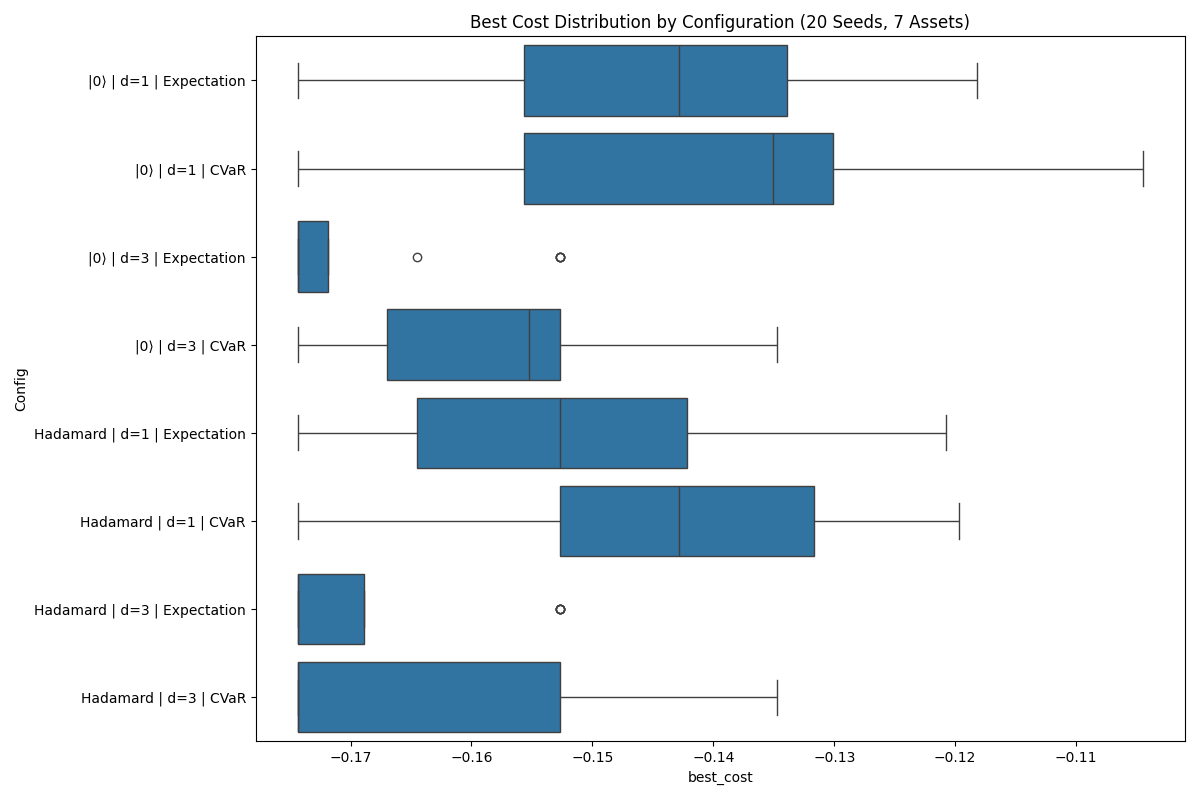
\includegraphics[width=\textwidth]{boxplot.png}
\caption{Distribution of best portfolio costs achieved across 20 independent seeds. Configurations are grouped by objective function, circuit depth, and initialization strategy. The red dashed line denotes the globally optimal portfolio cost $\mathcal{C}^* = -0.17435$.}
\label{fig:boxplot}
\end{figure}

\subsection{Effect of Initialization Strategy}

At circuit depth $d = 1$, Hadamard initialization achieves a slightly better mean best cost than $|0\rangle$ under both objectives: $-0.1508$ versus $-0.1453$ for Expectation, and $-0.1431$ versus $-0.1421$ for CVaR. It also exhibits lower variability ($0.0151$ vs.\ $0.0190$ for Expectation, $0.0159$ vs.\ $0.0203$ for CVaR), indicating more consistent convergence at shallow depth.
With only $d \times n = 7$ parameters, the circuit has limited ability to reshape the probability distribution independently of its initial state. These differences, however, are not statistically significant (Section~\ref{sec:stats}).

At $d = 3$, initialization stops mattering. Under Expectation, $|0\rangle$ edges out Hadamard by a small margin ($-0.1695$ vs.\ $-0.1689$, $r = 0.972$ vs.\ $0.969$), a margin small enough to call a tie. Under CVaR, though, Hadamard holds a real advantage over $|0\rangle$ ($-0.1645$ vs.\ $-0.1582$, $r = 0.944$ vs.\ $0.907$), and that four-point spread in $r$ is the largest initialization effect seen at this depth. So the choice of initial state is not irrelevant at $d=3$, it just depends on which objective is being optimized. With 21 parameters at depth 3, the ansatz appears to have enough capacity to reduce its dependence on the initial state.

\subsection{Effect of Circuit Depth}

Increasing depth from $d = 1$ to $d = 3$ improves mean best cost across all four combinations, at the cost of $3.5$--$4.0\times$ longer runtime and $2.4$--$2.7\times$ more function evaluations. The largest gain occurs for $|0\rangle$-Expectation: mean best cost improves from $-0.1453$ to $-0.1695$ ($r$ from $83.3\%$ to $97.2\%$). For Hadamard-CVaR, the gain is from $-0.1431$ to $-0.1645$ ($r$ from $82.1\%$ to $94.4\%$). A single layer provides only 7 rotation parameters and one entanglement round, tripling the depth to 21 parameters and three entanglement rounds substantially expands the expressible hypothesis space.

Figure~\ref{fig:convergence} plots the cumulative minimum objective value against COBYLA function evaluations, averaged across all $20$ seeds. The dominant visual separator is circuit depth, not initialization. Shallow $d=1$ runs flatten out early because the ansatz lacks the expressibility for COBYLA to keep improving after the first few evaluations. At $d=3$, the curves continue to descend well past that plateau and settle appreciably closer to the classical optimum before levelling off. Hadamard and $|0\rangle$ trajectories at the same depth, by contrast, lie nearly on top of each other throughout. In short, depth governs how close the optimizer can get, initialization mainly shapes the path taken to get there.

\begin{figure}[h!]
\centering
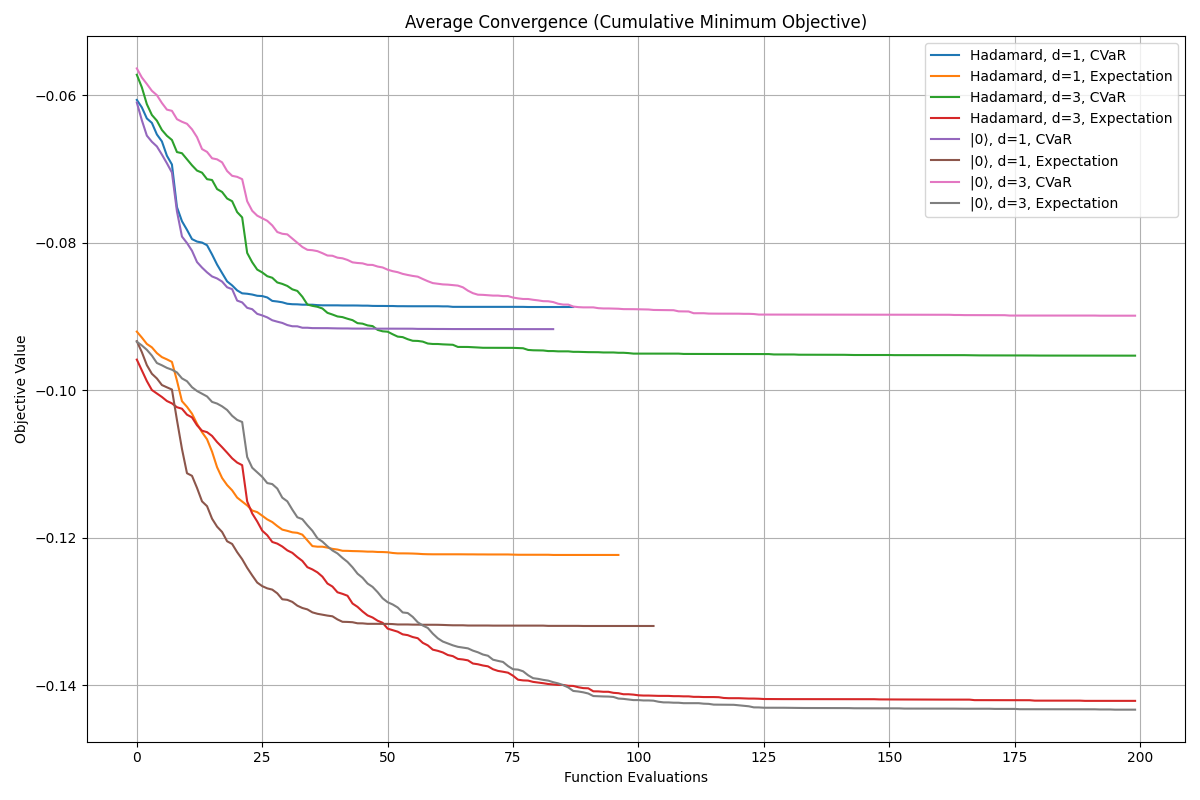
\includegraphics[width=\textwidth]{convergence.png}
\caption{Cumulative minimum objective value averaged over 20 seeds, plotted against COBYLA function evaluations. Each curve corresponds to one initialization--depth--objective configuration.}
\label{fig:convergence}
\end{figure}

\subsection{Statistical significance}
\label{sec:stats}
Table~\ref{tab:wilcoxon} reports Wilcoxon signed-rank test results for all three comparison families, paired by seed.

\begin{table}[h!]
\caption{Wilcoxon signed-rank test results on best cost, paired by seed ($n = 20$). Significance threshold: $p < 0.05$.}
\label{tab:wilcoxon}
\centering
\small
\setlength{\tabcolsep}{4pt}
\begin{tabular}{lccc}
\hline
\textbf{Comparison} & \textbf{$W$} & \textbf{$p$-value} & \textbf{Significant} \\
\hline
\multicolumn{4}{l}{\textit{Initialization: $|0\rangle$ vs.\ $H$}} \\
$d=1$, Exp  & 67.5 & 0.4330 & No \\
$d=1$, CVaR & 67.0 & 0.4204 & No \\
$d=3$, Exp  & 22.0 & 0.9489 & No \\
$d=3$, CVaR & 33.0 & 0.1233 & No \\
\hline
\multicolumn{4}{l}{\textit{Depth: $d=1$ vs.\ $d=3$}} \\
$H$, Exp           & 3.0  & 0.0008 & Yes \\
$H$, CVaR          & 8.0  & 0.0011 & Yes \\
$|0\rangle$, Exp   & 12.0 & 0.0013 & Yes \\
$|0\rangle$, CVaR  & 23.0 & 0.0064 & Yes \\
\hline
\multicolumn{4}{l}{\textit{Objective: Exp vs.\ CVaR}} \\
$H$, $d=1$         & 19.0 & 0.0355 & Yes \\
$H$, $d=3$         & 0.0  & 0.0431 & Yes \\
$|0\rangle$, $d=1$ & 34.0 & 0.6949 & No \\
$|0\rangle$, $d=3$ & 0.0  & 0.0014 & Yes \\
\hline
\end{tabular}
\end{table}

Across all four paired comparisons, initialization never reaches significance ($p \geq 0.123$). Hadamard and $|0\rangle$ do point in the same direction every time, yet with only 20 paired seeds the study may simply lack power to resolve an effect this small. Depth paints a sharply different picture: every comparison is significant by a comfortable margin ($p \leq 0.0064$), consistent with depth purchasing genuine expressive capacity rather than fitting noise. The objective-function comparisons occupy a middle ground. Three of four are nominally significant ($p \leq 0.0431$), but two of those sit close enough to the $0.05$ boundary ($p = 0.0355$, $p = 0.0431$) that they would plausibly be overturned by a multiple-comparisons correction, which has not been applied. The objective-function effect is therefore regarded as suggestive rather than established.

\subsection{Extended Experiments on a 12-Asset Universe}
\label{sec:extended}

To validate the findings on a larger problem instance, the experiments are extended to $n = 12$ U.S. equities (AAPL, MSFT, GOOG, AMZN, META, NVDA, TSLA, JPM, JNJ, V, PG, UNH) with circuit depths $d \in \{1, 2, 3, 4\}$, yielding $4 \times 2 \times 2 \times 20 = 320$ optimization runs. Both $n = 7$ and $n = 12$ remain classically tractable by exhaustive enumeration, these experiments therefore probe optimizer behaviour rather than quantum computational advantage. The classical optimum is obtained by evaluating all $2^{12} - 1 = 4095$ non-empty portfolios, giving $\mathcal{C}^* = -0.1642$. All other experimental parameters (optimizer, shots, seeds) are identical to the 7-asset setting.

Table~\ref{tab:s95_t95} reports the convergence metrics $S_{95}$ and $T_{95}$ for all 16 configurations.

\begin{table}[t]
\caption{Convergence metrics for the 12-asset experiments. $S_{95}$: fraction of 20 seeds reaching $r \geq 0.95$. $T_{95}$: mean iterations to first reach $r_k \geq 0.95$ over all 20 seeds, runs that do not reach the threshold are assigned $T_{95}=200$.}
\label{tab:s95_t95}
\centering
\begin{tabular}{lllcc}
\hline
\textbf{Init} & \textbf{$d$} & \textbf{Obj} & \textbf{$S_{95}$} & \textbf{$T_{95}$} \\
\hline
$H$         & 1 & Exp  & 0.05 & 128.2 \\
$H$         & 1 & CVaR & 0.00 & 132.8 \\
$H$         & 2 & Exp  & 0.60 & 21.0  \\
$H$         & 2 & CVaR & 0.20 & 45.2  \\
$H$         & 3 & Exp  & 0.45 & 28.1  \\
$H$         & 3 & CVaR & 0.20 & 39.6  \\
$H$         & 4 & Exp  & 0.60 & 8.2   \\
$H$         & 4 & CVaR & 0.35 & 8.4   \\
\hline
$|0\rangle$ & 1 & Exp  & 0.10 & 86.2  \\
$|0\rangle$ & 1 & CVaR & 0.05 & 124.2 \\
$|0\rangle$ & 2 & Exp  & 0.50 & 37.5  \\
$|0\rangle$ & 2 & CVaR & 0.10 & 64.5  \\
$|0\rangle$ & 3 & Exp  & 0.45 & 20.6  \\
$|0\rangle$ & 3 & CVaR & 0.25 & 41.0  \\
$|0\rangle$ & 4 & Exp  & 0.45 & 7.1   \\
$|0\rangle$ & 4 & CVaR & 0.40 & 5.5   \\
\hline
\end{tabular}
\end{table}

\subsection{Convergence Analysis}

Among the factors varied in this study, circuit depth has the largest effect on convergence speed. At $d = 1$, virtually no configuration reaches 95\% optimality within 200 iterations: $S_{95} \leq 0.10$ across all initializations and objectives, with $T_{95}$ exceeding 86 iterations on average (note that at such low $S_{95}$, $T_{95}$ is dominated by the 200-iteration ceiling and should not be interpreted as a genuine convergence time). Depth pays off along two distinct axes, and they do not move together. Success rate shows diminishing returns, convergence speed shows accelerating returns. The largest jump occurs between $d=1$ and $d=2$: parameter count doubles from 12 to 24, a second entanglement round is added, and circuit expressibility increases correspondingly. Beyond $d=2$, additional depth contributes little further to success rate, its primary effect is to reduce the number of iterations required for seeds that do converge.

$S_{95}$ is not monotonic in depth, and this warrants direct comment. For Hadamard-Expectation it follows $0.60 \to 0.45 \to 0.60$ across $d = 2, 3, 4$, $|0\rangle$-Expectation shows a comparable dip, $0.50 \to 0.45 \to 0.45$. We do not interpret this as a genuine depth effect. With only 20 seeds per configuration, fluctuations of this magnitude are consistent with sampling variability, and attributing them to depth would overfit a small sample. The convergence-speed result is more robust: at $d=4$, seeds that reach 95\% optimality do so within 5--8 iterations on average, across configurations spanning $S_{95} = 0.35$--$0.60$.

\subsection{Effect of Circuit Depth on Convergence}
Success rate and convergence speed respond to depth differently: the former shows diminishing returns while the latter accelerates. The sharpest transition lies between $d = 1$ and $d = 2$, where the parameter count doubles from 12 to 24 and a second entanglement round enters the circuit, materially boosting expressibility. Past $d = 2$, adding layers chiefly accelerates how fast converging seeds reach the target, without appreciably raising the share of seeds that converge at all. $S_{95}$ does not grow monotonically with depth everywhere, for Hadamard-Expectation it follows 0.60 at $d = 2$, dips to 0.45 at $d = 3$, then recovers to 0.60 at $d = 4$, $|0\rangle$-Expectation exhibits a comparable dip (0.50 $\to$ 0.45 $\to$ 0.45). Given that each configuration has only 20 seeds, fluctuations of this size are compatible with sampling noise and should not be over-read. At $d = 4$, those seeds that do reach 95\% optimality do so in roughly 5--8 iterations ($S_{95} = 0.35$--$0.60$).

\subsection{Expectation versus CVaR}
At $d = 2$ with Hadamard initialization, $S_{95}^{\text{Exp}} = 0.60$ versus $S_{95}^{\text{CVaR}} = 0.20$, at $d = 4$, $S_{95}^{\text{Exp}} = 0.60$ versus $S_{95}^{\text{CVaR}} = 0.35$. The Wilcoxon results from the 12-asset runs show significant differences between Expectation and CVaR at $d = 1$ ($p = 0.0006$--$0.0049$) and $d = 2$ ($p = 0.0005$--$0.0012$), with significance diminishing at greater depths ($d = 3$: $p = 0.068$--$0.133$, $d = 4$: $p = 0.021$--$0.127$).

CVaR's lower success rate is consistent with its tail-focused evaluation: restricting the objective to the highest-cost $\alpha = 0.3$ fraction of sampled outcomes uses only part of the measurement distribution, which can produce a noisier objective estimate and complicate COBYLA's local search within the 200-iteration budget. CVaR's success rate is non-decreasing with depth in both initialization settings, although the present experiments do not establish whether increased expressibility is the direct cause.
Figures~\ref{fig:boxplot_12}--\ref{fig:s95_depth} present the distribution of approximation ratios, mean convergence trajectories, iterations to 95\% optimality, and success rate as a function of circuit depth for the 12-asset experiments.
\begin{figure}[h!]
\centering
\includegraphics[width=\textwidth]{boxplots.png}
\caption{Distribution of approximation ratios across 20 seeds for the 12-asset experiments. Configurations are grouped by initialization, depth, and objective. The dashed lines mark $r = 1.0$ (global optimum) and $r = 0.95$ (convergence target).}
\label{fig:boxplot_12}
\end{figure}
\begin{figure}[h!]
\centering
\includegraphics[width=\textwidth]{convergence_curves.png}
\caption{Cumulative best approximation ratio $r_k$ averaged over 20 seeds, plotted against function evaluations for the 12-asset experiments. Horizontal lines indicate the global optimum ($r = 1.0$) and the 95\% convergence target ($r = 0.95$).}
\label{fig:convergence_12}
\end{figure}
\begin{figure}[h!]
\centering
\includegraphics[width=\textwidth]{t95_vs_depth.png}
\caption{Mean iterations to 95\% optimality ($T_{95}$) as a function of circuit depth for the 12-asset experiments, stratified by initialization and objective.}
\label{fig:t95_depth}
\end{figure}
\begin{figure}[h!]
\centering
\includegraphics[width=\textwidth]{success_rate_vs_depth.png}
\caption{Success rate $S_{95}$ (fraction of seeds achieving $r \geq 0.95$) as a function of circuit depth for the 12-asset experiments, stratified by initialization and objective.}
\label{fig:s95_depth}
\end{figure}

\subsection{Discussion}

Of the three factors examined, circuit depth exerts the strongest and most reproducible influence on optimization quality. A single-layer circuit ($d = 1$) contains only $n$ free parameters and one entanglement round, which tightly constrains how far the optimizer can move the output distribution away from its starting point. The modest edge that Hadamard initialization shows at shallow depth plausibly stems from the uniform superposition seeding probability across the full $2^n$-dimensional basis, whereas $|0\rangle$ concentrates all amplitude on one basis state. When the parameter budget is small, that broader starting distribution may let the optimizer sample favourable portfolios sooner. No direct measurement of probability flow within the circuit was performed, so this account remains interpretive rather than mechanistic. At $d = 3$ the ansatz carries $3n$ parameters and three entanglement rounds, markedly expanding its expressibility. With that much capacity the circuit can sculpt intricate probability distributions largely irrespective of where it started, and the initial state correspondingly loses influence. This is consistent with the Expectation results, where $|0\rangle$ and Hadamard perform similarly. The larger parameter space appears to offer enough distinct pathways to the optimum that initialization is less limiting. Under CVaR, Hadamard retains a small empirical advantage at $d = 3$, though it is not statistically significant. A possible explanation is that the uniform superposition exposes the optimizer to a broader set of portfolio configurations early in the optimization. This may affect the tail distribution used by the CVaR objective. This explanation remains tentative because the initialization difference is not statistically significant.

All initialization comparisons remain non-significant under the Wilcoxon test ($p \geq 0.123$ for $n = 7$, $p \geq 0.243$ for $n = 12$). Initialization produces directional shifts early in optimization, but among the factors varied here, circuit depth has the largest effect on solution quality.

It is worth stressing that the two initialization strategies do not correspond to distinct circuit architectures. Under the real-amplitude ansatz used here ($R_Y$ rotations with CNOT entanglement), adding Hadamard gates before the variational layers leaves the parameter count and layer structure unchanged, only the starting state differs. Observed performance gaps are therefore better ascribed to altered optimization trajectories than to any change in representational power---a reading that aligns with the non-significant Wilcoxon outcomes.
The 12-asset experiments quantify this depth dependence through convergence metrics. $T_{95}$ shows a diminishing-returns pattern, the largest change occurs between $d = 1$ and $d = 2$, where $T_{95}$ drops from $\sim$86--133 to $\sim$21--65 iterations (the $d = 1$ values are ceiling-dominated and do not represent genuine convergence times), further increases to $d = 3$ and $d = 4$ yield progressively smaller gains, with $T_{95}$ reaching $\sim$5--8 iterations at $d = 4$. $S_{95}$ shows a similar threshold effect from $d = 1$ to $d = 2$, jumping from 0.00--0.10 to 0.20--0.60, while the changes from $d = 2$ to $d = 4$ are smaller and not strictly monotonic.

Expectation's advantage over CVaR in the 12-asset setting is most evident in $S_{95}$, which is higher for Expectation at every depth. $T_{95}$ is generally lower for Expectation, although CVaR converges faster at $d=4$ for $|0\rangle$ initialization ($5.5$ vs.\ $7.1$ iterations). The lower success rates observed for the tail-focused objective are consistent with its reliance on only a subset of sampled outcomes, although the present experiments do not isolate estimator variance as the cause.

A few limitations apply. All experiments were run using the Qiskit Aer shot-based simulator (\texttt{AerSimulator}) \cite{qiskitAer}, without including gate errors, decoherence, or readout noise, on physical hardware these noise sources could interact with initialization differently. The asset universe is restricted to $n \leq 12$ equities, for which the classical optimum is obtainable by exhaustive enumeration, these experiments therefore characterize optimizer behaviour rather than demonstrating quantum advantage, and scaling to $n = 20$--$30$ assets would test whether the observed trends hold where classical enumeration becomes impractical. Only one ansatz architecture ($R_Y$ rotations with linear CNOT entanglement) and one optimizer (COBYLA) are evaluated, the convergence conclusions may be optimizer-specific, and alternative ans\"atze or optimizers may respond differently to initialization. The fixed COBYLA budget of 200 iterations may penalize deeper circuits with more parameters, adaptive budgets scaled to parameter count should be considered in future work.

Future work should test the initialization strategies on noisy quantum hardware, extend the asset universe beyond the range where exhaustive classical enumeration is feasible, and compare different ansatz architectures and optimizers. It would also be useful to investigate initialization schemes that use properties of the cost Hamiltonian, including QAOA and problem-specific circuits, to clarify whether the initialization--depth--objective interaction is ansatz-dependent, and adaptive initialization schemes where the starting state is chosen based on properties of the cost Hamiltonian.
\section{Conclusion}\label{conclusion}

This study compares \emph{qubit} initialization strategies Hadamard \cite{nielsen2010} versus computational zero-state $|0\rangle$ in variational quantum portfolio optimization. Experiments covered 7 and 12 U.S. equities under two objective functions (Expectation and CVaR). The 7-asset experiment uses circuit depths $d \in \{1,3\}$, while the 12-asset experiment uses $d \in \{1,2,3,4\}$, with 20 independent random seeds, yielding 160 and 320 runs, respectively.

The main result is that circuit depth has a strong effect on solution quality ($p \leq 0.0064$), while initialization strategy does not reach significance at either problem scale. The study may be underpowered to detect small initialization effects, so the null results should not be taken as evidence that initialization has no effect whatsoever. At $d = 1$, Hadamard initialization produces slightly lower mean cost and variance under both objectives, suggesting more stable optimization when the ansatz has limited expressibility, but these differences are not statistically significant.

The 12-asset experiments confirm these results at a larger scale and extend the analysis through the convergence metrics $T_{95}$ and $S_{95}$. The largest improvement in both success rate and convergence speed occurs between $d = 1$ and $d = 2$, further increases in depth mainly accelerate convergence rather than expand the fraction of successful seeds. Expectation achieves higher success rates ($S_{95}$ up to 0.60 vs.\ 0.35 at $d = 4$). Differences in $T_{95}$ at $d = 4$ are comparatively small (approximately 5--8 iterations across both objectives) and should be interpreted together with the corresponding success rates.

For the ansatz and optimizer studied here, circuit depth has a larger effect on optimization performance than the choice of initialization. In these experiments, the transition from $d = 1$ to $d = 2$ produces the first substantial improvement in optimization performance. All results are from ideal noiseless simulation, the behavior of initialization strategies on physical quantum processors remains open. Future work should include evaluation on noisy hardware, scaling to asset universes where classical enumeration becomes infeasible, testing additional optimizers to determine whether convergence conclusions are optimizer-specific, and comparison across ansatz architectures to test the generality of these observations.

\begin{credits}
\subsubsection{\discintname}
The author has no competing interests to declare that are relevant to the content of this article.
\end{credits}

\begin{thebibliography}{99}
\bibitem{nielsen2010}
M. A. Nielsen and I. L. Chuang, \textit{Quantum Computation 
and Quantum Information}. Cambridge: Cambridge University 
Press, 2010.
\bibitem{rockafellar2000}
R. T. Rockafellar and S. Uryasev, ``Optimization of conditional 
value-at-risk,'' \textit{Journal of Risk}, vol. 2, no. 3, 
pp. 21--41, 2000.
\bibitem{markowitz1952}
H. Markowitz, ``Portfolio selection,'' \textit{The Journal 
of Finance}, vol. 7, no. 1, pp. 77--91, 1952.
\bibitem{barkoutsos2020}
P. K. Barkoutsos, G. Nannicini, A. Robert, I. Tavernelli, 
and S. Woerner, ``Improving variational quantum optimization 
using CVaR,'' \textit{Quantum}, vol. 4, p. 256, 2020.
\bibitem{scursulim2026}
J. V. S. Scursulim, G. M. Langeloh, V. L. Beltran, and
S. Brito, ``Multiclass portfolio optimization via variational
quantum Eigensolver with Dicke state ansatz,''
\textit{Scientific Reports}, vol. 16, no. 1, p. 6208, 2026.
\bibitem{powell1994}
M. J. D. Powell, ``A direct search optimization method 
that models the objective and constraint functions by 
linear interpolation,'' in \textit{Advances in 
Optimization and Numerical Analysis}. Dordrecht: 
Springer, 1994, pp. 51--67.
\bibitem{kandala2017hardware}
A. Kandala \textit{et al.}, ``Hardware-efficient variational quantum eigensolver for small molecules and quantum magnets,'' \textit{Nature}, vol. 549, no. 7671, pp. 242--246, 2017.
\bibitem{mcclean2018barren}
J. R. McClean \textit{et al.}, ``Barren plateaus in quantum neural network training landscapes,'' \textit{Nature Communications}, vol. 9, p. 4812, 2018.
\bibitem{Wurtz_2021_fixed_angle}
J. Wurtz and D. Lykov, ``Fixed-angle conjectures for the quantum approximate optimization algorithm on regular MaxCut graphs,'' \textit{Physical Review A}, vol. 104, no. 5, p. 052419, 2021.
\bibitem{qiskitAer}
Qiskit Aer, ``Qiskit Aer documentation,'' Qiskit, 2026.
[Online]. Available: https://qiskit.github.io/qiskit-aer/
\bibitem{yfinance}
R. Aroussi, ``yfinance: Download market data from Yahoo! Finance's API,'' GitHub repository, 2026. [Online]. Available: https://github.com/ranaroussi/yfinance
\bibitem{cerezo2021variational}
M. Cerezo \textit{et al.}, ``Variational quantum algorithms,''
\textit{Nature Reviews Physics}, vol. 3, no. 9, pp. 625--644, 2021.

\bibitem{peruzzo2014vqe}
A. Peruzzo, J. McClean, P. Shadbolt, M.-H. Yung, X.-Q. Zhou,
P. J. Love, A. Aspuru-Guzik, and J. L. O'Brien,
``A variational eigenvalue solver on a photonic quantum processor,''
\textit{Nature Communications}, vol. 5, p. 4213, 2014.

\bibitem{preskill2018nisq}
J. Preskill, ``Quantum computing in the NISQ era and beyond,''
\textit{Quantum}, vol. 2, p. 79, 2018.

\bibitem{egger2021warmstart}
D. J. Egger, J. Mare\v{c}ek, and S. Woerner,
``Warm-starting quantum optimization,''
\textit{Quantum}, vol. 5, p. 479, 2021.

\bibitem{orus2019finance}
R. Or\'us, S. Mugel, and E. Lizaso,
``Quantum computing for finance: Overview and prospects,''
\textit{Reviews in Physics}, vol. 4, p. 100028, 2019.

\bibitem{egger2020finance}
D. J. Egger, C. Gambella, J. Marecek, S. McFaddin, M. Mevissen,
R. Raymond, A. Simonetto, S. Woerner, and E. Yndurain,
``Quantum computing for finance: State-of-the-art and future prospects,''
\textit{IEEE Transactions on Quantum Engineering}, vol. 1, pp. 1--24, 2020.

\bibitem{kerenidis2019portfolio}
I. Kerenidis, A. Prakash, and D. Szil\'agyi,
``Quantum algorithms for portfolio optimization,''
in \textit{Proceedings of the 1st ACM Conference on Advances in Financial Technologies},
2019, pp. 147--155.

\bibitem{zhou2020qaoa}
L. Zhou, S.-T. Wang, S. Choi, H. Pichler, and M. D. Lukin,
``Quantum approximate optimization algorithm: Performance, mechanism,
and implementation on near-term devices,''
\textit{Physical Review X}, vol. 10, no. 2, p. 021067, 2020.

\bibitem{mugel2022dynamic}
S. Mugel, C. Kuchkovsky, E. S\'anchez, S. Fern\'andez-Lorenzo,
J. Luis-Hita, E. Lizaso, and R. Or\'us,
``Dynamic portfolio optimization with real datasets using quantum processors
and quantum-inspired tensor networks,''
\textit{Physical Review Research}, vol. 4, p. 013006, 2022.
\end{thebibliography}

\end{document}